\documentclass[a4paper,
fontsize=11pt,
%headings=small,
oneside,
numbers=noperiodatend,
parskip=half-,
bibliography=totoc,
final
]{scrartcl}

\usepackage{synttree}
\usepackage{graphicx}
\setkeys{Gin}{width=.37\textwidth} %default pics size

\graphicspath{{./plots/}}
\usepackage[ngerman]{babel}
\usepackage[T1]{fontenc}
%\usepackage{amsmath}
\usepackage[utf8x]{inputenc}
\usepackage [hyphens]{url}
\usepackage{booktabs} 
\usepackage[left=2.4cm,right=2.4cm,top=2.3cm,bottom=2cm,includeheadfoot]{geometry}
\usepackage{eurosym}
\usepackage{multirow}
\usepackage[ngerman]{varioref}
\setcapindent{1em}
\renewcommand{\labelitemi}{--}
\usepackage{paralist}
\usepackage{pdfpages}
\usepackage{lscape}
\usepackage{float}
\usepackage{acronym}
\usepackage{eurosym}
\usepackage[babel]{csquotes}
\usepackage{longtable,lscape}
\usepackage{mathpazo}
\usepackage[normalem]{ulem} %emphasize weiterhin kursiv
\usepackage[flushmargin,ragged]{footmisc} % left align footnote
\usepackage{ccicons} 

%%%% fancy LIBREAS URL color 
\usepackage{xcolor}
\definecolor{libreas}{RGB}{112,0,0}

\usepackage{listings}

\urlstyle{same}  % don't use monospace font for urls

\usepackage[fleqn]{amsmath}

%adjust fontsize for part

\usepackage{sectsty}
\partfont{\large}

%Das BibTeX-Zeichen mit \BibTeX setzen:
\def\symbol#1{\char #1\relax}
\def\bsl{{\tt\symbol{'134}}}
\def\BibTeX{{\rm B\kern-.05em{\sc i\kern-.025em b}\kern-.08em
    T\kern-.1667em\lower.7ex\hbox{E}\kern-.125emX}}

\usepackage{fancyhdr}
\fancyhf{}
\pagestyle{fancyplain}
\fancyhead[R]{\thepage}

% make sure bookmarks are created eventough sections are not numbered!
% uncommend if sections are numbered (bookmarks created by default)
\makeatletter
\renewcommand\@seccntformat[1]{}
\makeatother


\usepackage{hyperxmp}
\usepackage[colorlinks, linkcolor=black,citecolor=black, urlcolor=libreas,
breaklinks= true,bookmarks=true,bookmarksopen=true]{hyperref}
%URLs hart brechen
\makeatletter 
\g@addto@macro\UrlBreaks{ 
  \do\a\do\b\do\c\do\d\do\e\do\f\do\g\do\h\do\i\do\j 
  \do\k\do\l\do\m\do\n\do\o\do\p\do\q\do\r\do\s\do\t 
  \do\u\do\v\do\w\do\x\do\y\do\z\do\&\do\1\do\2\do\3 
  \do\4\do\5\do\6\do\7\do\8\do\9\do\0} 
% \def\do@url@hyp{\do\-} 
\makeatother 

%meta
%meta

\fancyhead[L]{W. Horstmann\\ %author
LIBREAS. Library Ideas, 34 (2018). % journal, issue, volume.
\href{http://nbn-resolving.de/}
{}} % urn 
% recommended use
%\href{http://nbn-resolving.de/}{\color{black}{urn:nbn:de...}}
\fancyhead[R]{\thepage} %page number
\fancyfoot[L] {\ccLogo \ccAttribution\ \href{https://creativecommons.org/licenses/by/3.0/}{\color{black}Creative Commons BY 3.0}}  %licence
\fancyfoot[R] {ISSN: 1860-7950}

\title{\LARGE{Der vorausgeworfene Schatten des Professor Dziatzko}}% title
\author{Wolfram Horstmann} % author

\setcounter{page}{1}

\hypersetup{%
      pdftitle={Der vorausgeworfene Schatten des Professor Dziatzko},
      pdfauthor={Wolfram Horstmann},
      pdfcopyright={CC BY 3.0 Unported},
      pdfsubject={LIBREAS. Library Ideas, 34 (2018).},
      pdfkeywords={Bibliothekswissenschaft, Geschichte, Bibliographie},
      pdflicenseurl={https://creativecommons.org/licenses/by/3.0/},
      pdfcontacturl={http://libreas.eu},
      baseurl={http://libreas.eu},
      pdflang={de},
      pdfmetalang={de}
     }



\date{}
\begin{document}

\maketitle
\thispagestyle{fancyplain} 

%abstracts

%body
\emph{Großer Dank gebührt Dr.~Christian Fieseler von der SUB Göttingen
und Dr.~Holger Berwinkel vom Universitätsarchiv in Göttingen für die
Aufarbeitung und Bereitstellung der historischen Informationen in diesem
Beitrag.}

\begin{quote}
\enquote{Es ist mit erfreulich, Euer Hochwohlgeboren im Verfolg meines
Erlasses vom 22. Juli d{[}iesen{]} J{[}ahres{]} {[}\ldots{}{]} davon in
Kenntniß zu setzen, daß Seine Majestät der Kaiser und König
Allergnädigst geruht haben, Sie zum ordentlichen Professor in der
philosophischen Fakultät der Universität Göttingen zu ernennen. Indem
ich Ihnen die darüber ausgefertigte, unterm 15. August d. J.
Allerhöchsten Orts vollzogene Bestallung beifolgend übersende, verleihe
ich Ihnen in der genannten Fakultät das {[}...{]} Ordinariat mit dem
Bemerken, daß ich mir wegen Ertheilung eines Lehrauftrages die Verfügung
einstweilen vorbehalte.} {[}Schreiben aus dem Ministerium der
geistlichen, Unterrichts- und Medicinalangelegenheiten an Karl Dziatzko
vom 26. August 1886. Aus Dziatzkos Personalakte (Kur. Nr. 5961 ), der zu
der Zeit Oberbibliothekar in Göttingen war.{]}
\end{quote}

\begin{center}
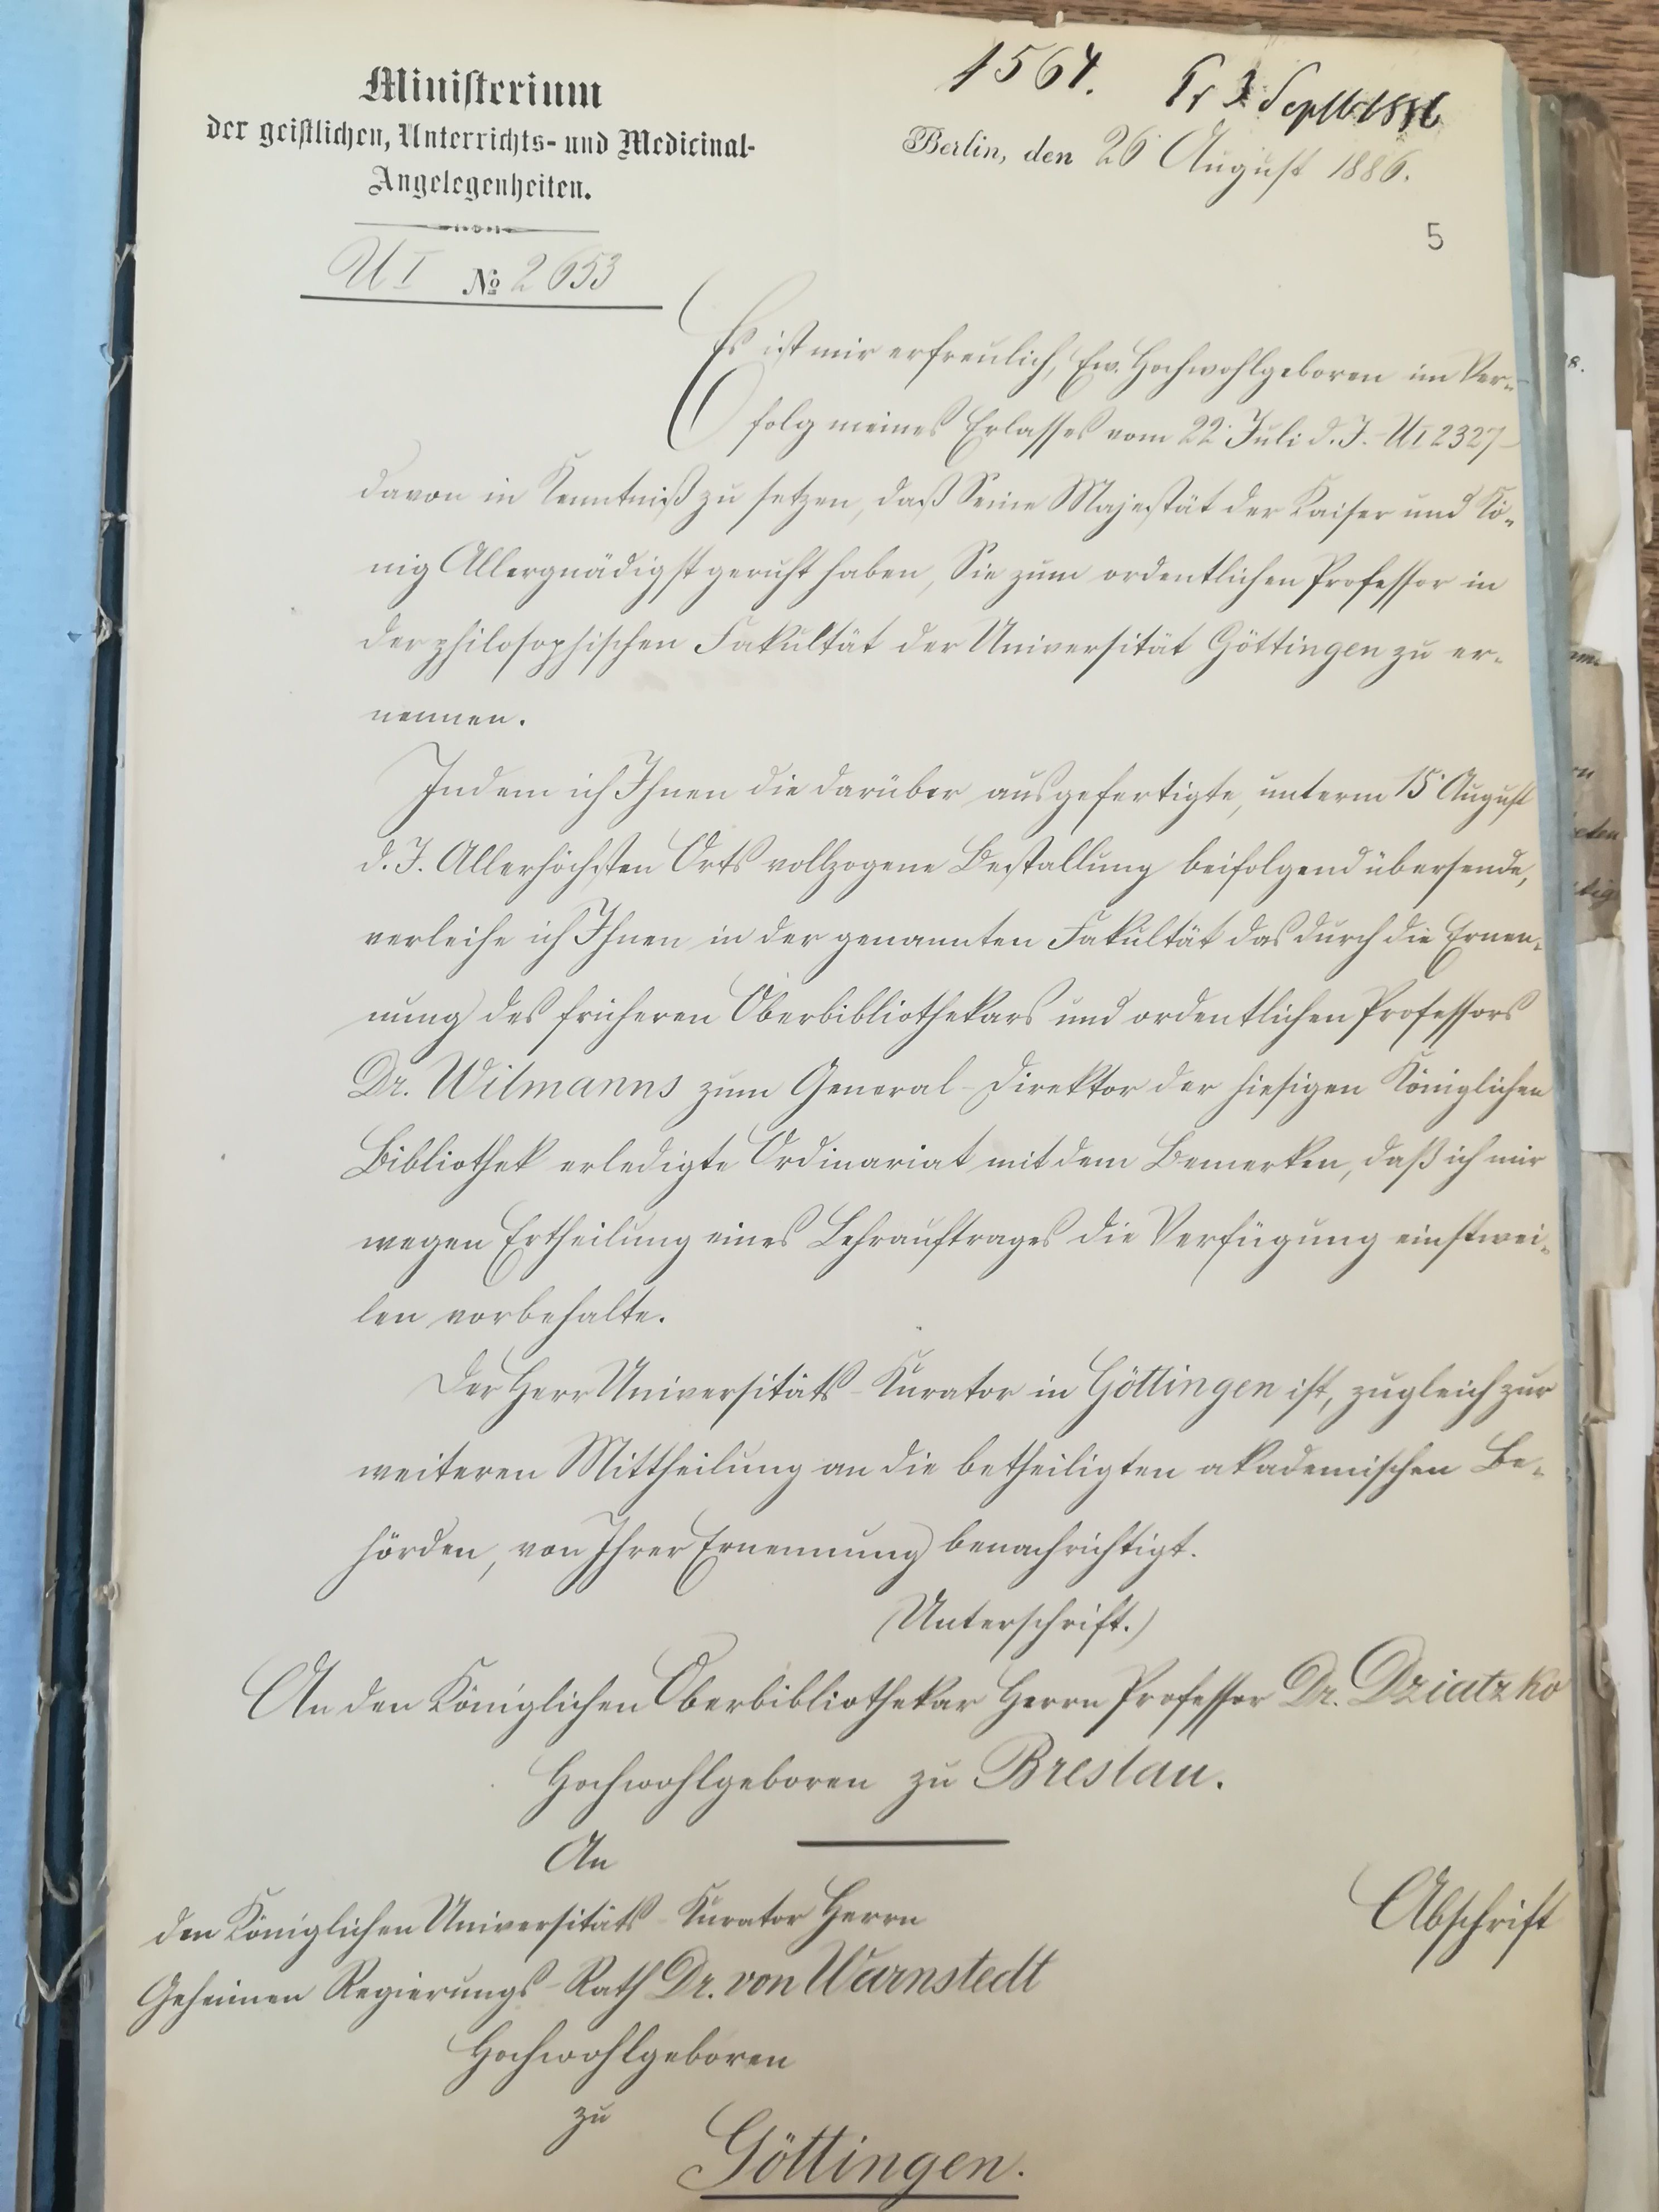
\includegraphics{img/image1.jpg}
\end{center}

Die Entstehungsgeschichte des Instituts für Bibliotheks- und
Informationswissenschaft der Humboldt"=Universität zu Berlin ist eng mit
der Universität Göttingen verbunden. Wie in der vorbildlichen
Ausarbeitung von Renate Rohde\footnote{Renate Rohde. Zur Geschichte der
  bibliothekswissenschaftlichen Ausbildung in Berlin.
  \url{https://www.ibi.hu-berlin.de/de/institut/leitbild/gesch-ausbildung/gesch-ausbildung}}
bereits gezeigt, wurde 1886/1887 zunächst ein Lehrstuhl in Göttingen
eingerichtet. Zum Jubiläum des IBI sollen einige Aushebungen ergänzt
werden.

Erster Inhaber des Lehrstuhls war der derzeitige Oberbibliothekar
(Bibliotheksdirektor) Karl Dziatzko. Hätte Karl Dziatzko gedacht, dass
mehr als 125 Jahre später drei Generationen Göttinger
Bibliotheksdirektoren als Professoren gleichzeitig an einem Berliner
Institut aktiv sind? Er konnte ja nicht wissen, dass der Göttinger
Lehrstuhl 1921 nach Berlin verlagert werden sollte. Oder wusste er es
doch? Bemerkenswert ist, dass einige Traditionen schon damals angelegt
waren, wie in einem weiteren Schreiben vom 6. Oktober 1886 deutlich
wird:

\begin{quote}
\enquote{Im Verfolg meines Erlasses vom 26. August d. J. {[}\ldots{}{]}
betreffend Ihre Ernennung zum ordentlichen Professor in der
philosophischen Fakultät der dortigen Universität, ertheile ich Euer
Hochwohlgeboren hiermit den Lehrauftrag, Vorlesungen und Übungen über
Bibliotheks-Hülfswissenschaften zu halten, wobei ich indeß Ihrem Wunsche
gemäß voraussetze, daß der Umfang Ihrer Lehrtätigkeit sich auf 3 bis 4
Stunden wöchentlich beschränken wird, indem, wie ich gerne anmerke, Ihre
Hauptarbeit der Verwaltung der Universitäts-Bibliothek gewidmet sein
muß.}
\end{quote}

\begin{center}
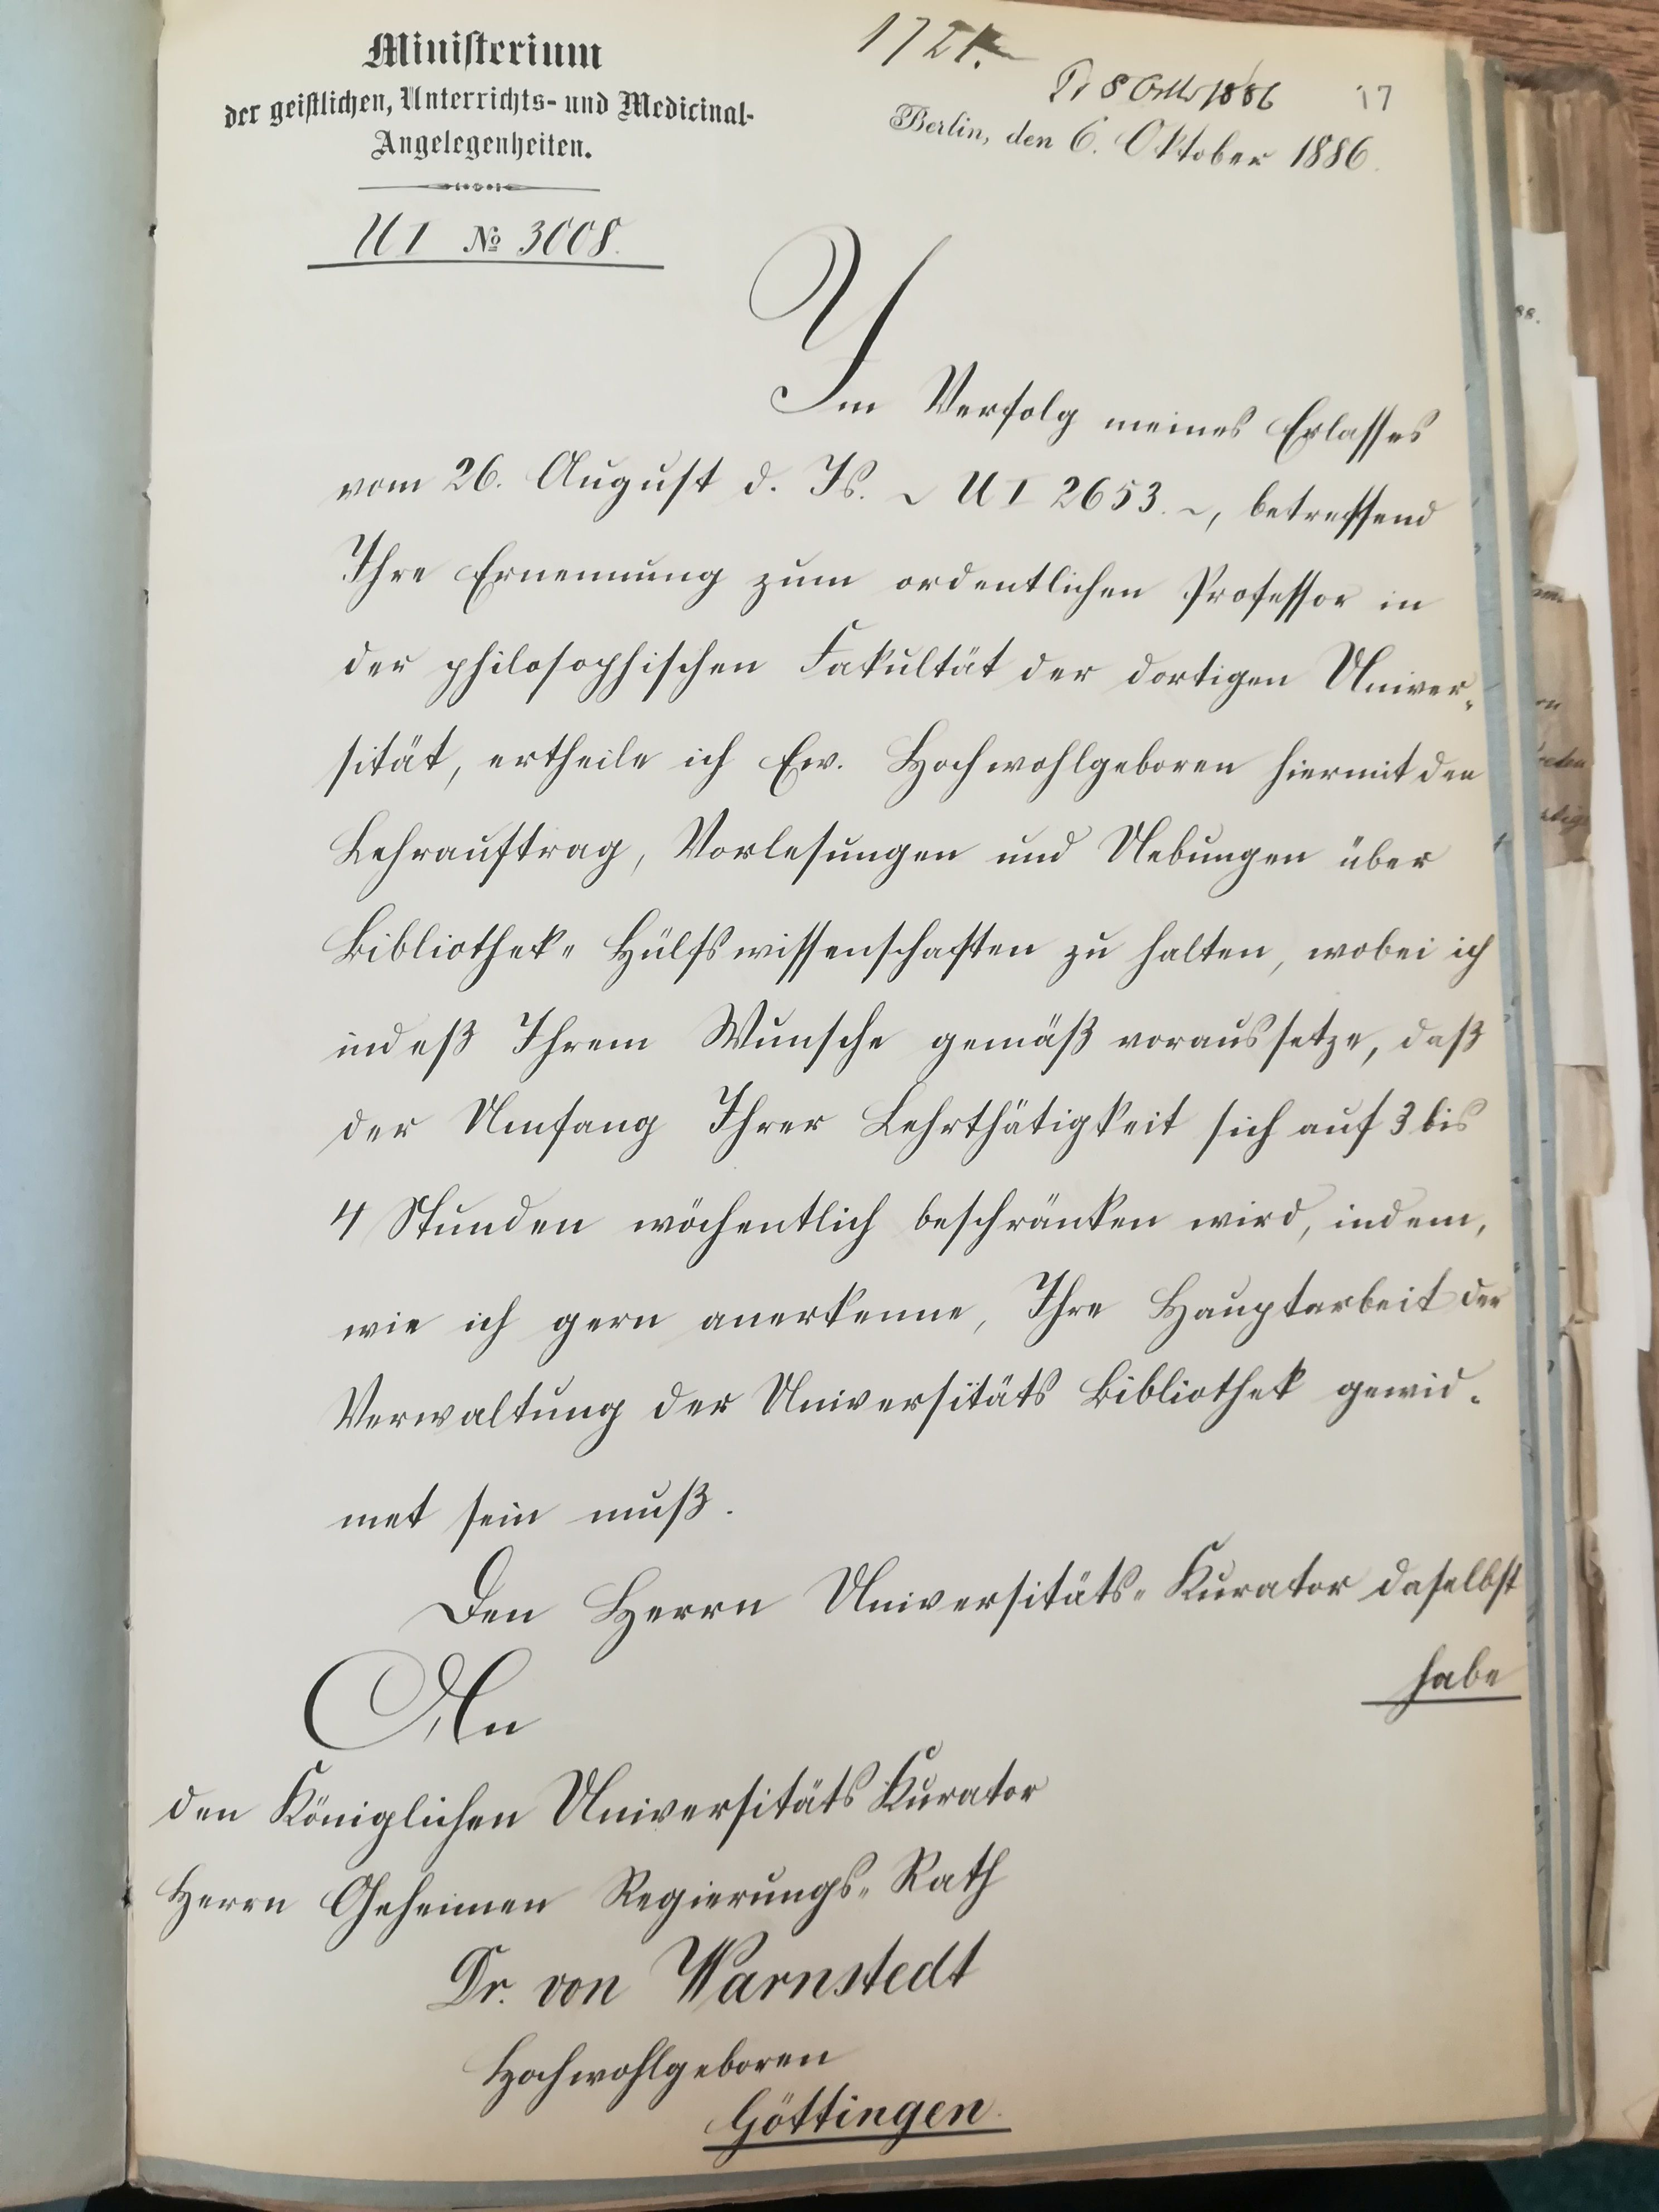
\includegraphics{img/image2.jpg}
\end{center}

Die drei heutigen Göttinger Professoren am IBI erleben in der Tat das
gleiche Schicksal einer Doppelrolle und eines eingeschränkten
Lehrumfangs, die Karl Dziatzko offensichtlich bereits 1886 formuliert
hat. Einige Dinge in Wissenschaft und Bibliothekswesen ändern sich
offenbar gar nicht. Aber wie hätte sich \enquote{elektronisches
Publizieren} oder \enquote{digitale Geisteswissenschaft} in Karl
Dziatzkos Ohren angehört -- eingedenk des Umstandes, dass H.G. Wells zu
dieser Zeit vielleicht gerade einmal die ersten Ideen zur
\enquote{Zeitmaschine} im Kopf spukten? Oder gibt es eine geheime
Verbindung zwischen Zukunftsvorhersagen und Bibliothek? (Immerhin
schrieb auch Ray Bradbury \enquote{Fahrenheit 451} im Keller der
Powell-Bibliothek der University of California, Los Angeles.)

Die Suche nach weiteren versteckten Anzeichen einer Verbindung von
Bibliothek zu Zukunftsvorhersagen bestätigt sich zunächst nicht. Der
ministerielle Erlass wurde nüchtern zum Beginn des Haushaltsjahres
1887/1888 umgesetzt. (Von einer weiteren Aufarbeitung des Datums
\enquote{1. April} soll an dieser Stelle abgesehen werden.)

\begin{quote}
\enquote{Im Verfolg des Curatorial-Erlasses vom 6. September
v{[}origen{]} J{[}ahres{]} No.~1564 benachrichtige ich die
philosophische Fakultät, daß der Herr Minister der geistlichen
pp.~Angelegenheiten zufolge hohen Rescripts vom 9./11. d{[}es{]}
M{[}ona{]}ts die durch den Staatshaushalts-Etat für 1. April 1887/8 bei
der hiesigen Universität begründete ordentliche Professur für
Bibliotheks-Hülfswissenschaften dem ordentlichen Professor und
Oberbibliothekar Dr.~Dziatzko hieselbst vom 1. April d{[}es{]}
J{[}ahres{]} ab verliehen hat.} {[}Universitäts-Curatorium No.~642,
Göttingen, den 12. April 1887{]}
\end{quote}

\begin{center}
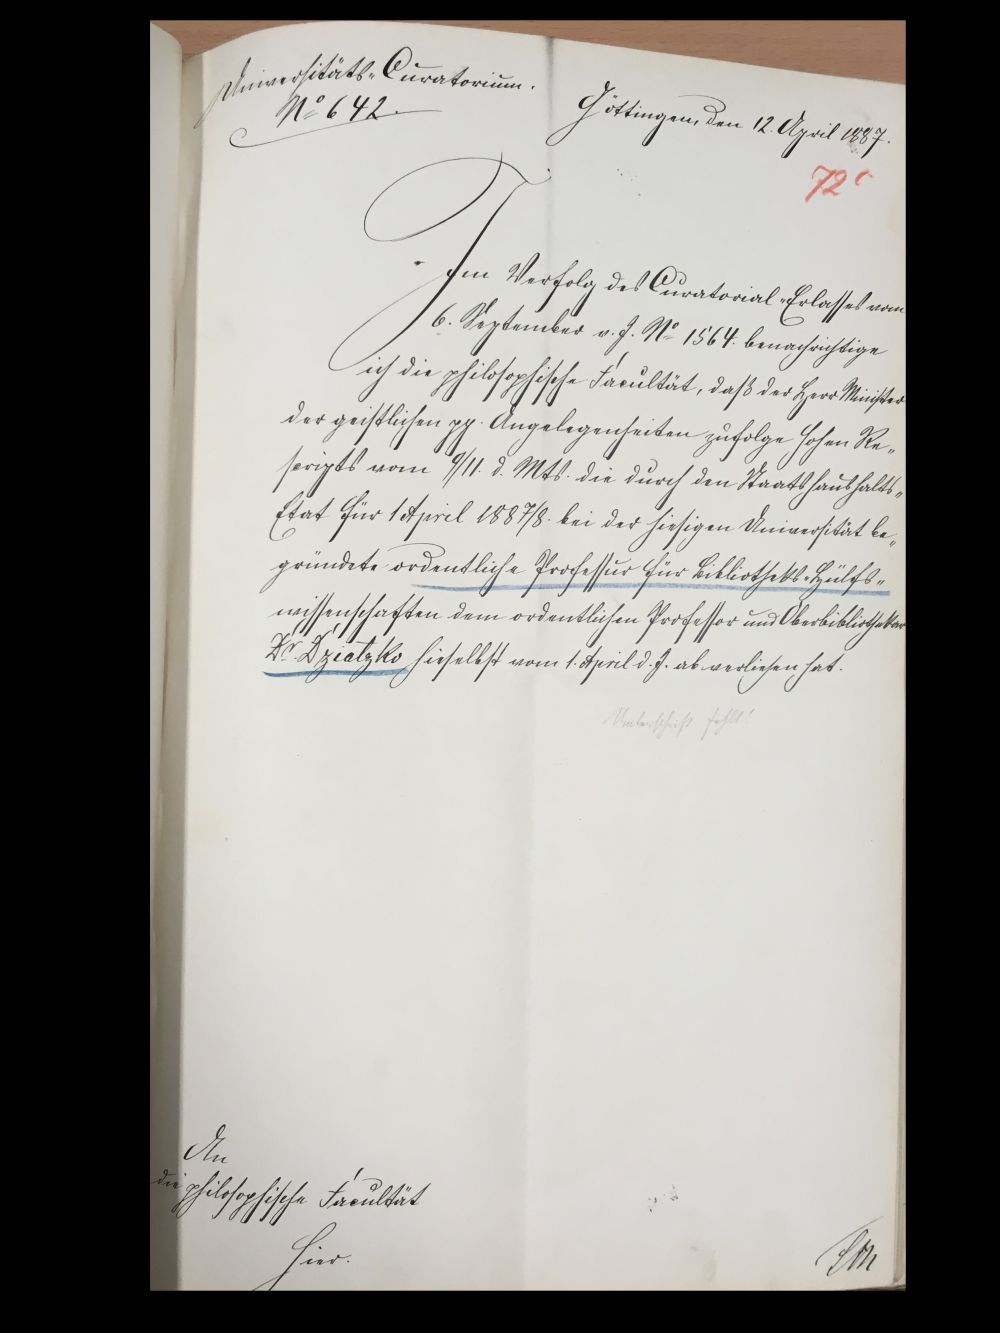
\includegraphics{img/image3.jpg}
\end{center}

Auch die erste Lehrveranstaltung Karl Dziatzkos deutet nicht auf
wahrsagerische Verwicklungen. Im Vorlesungsverzeichnis der Universität
Göttingen heißt es unter Literatur- und Kunstgeschichte:

\begin{quote}
\emph{\enquote{Bibliotheksverwaltungslehre: Dienst. und Freit. 8 Uhr, im
Anschluss Übungen (unentgeltlich). Zeit vorbehalten.}}
\end{quote}

\begin{center}
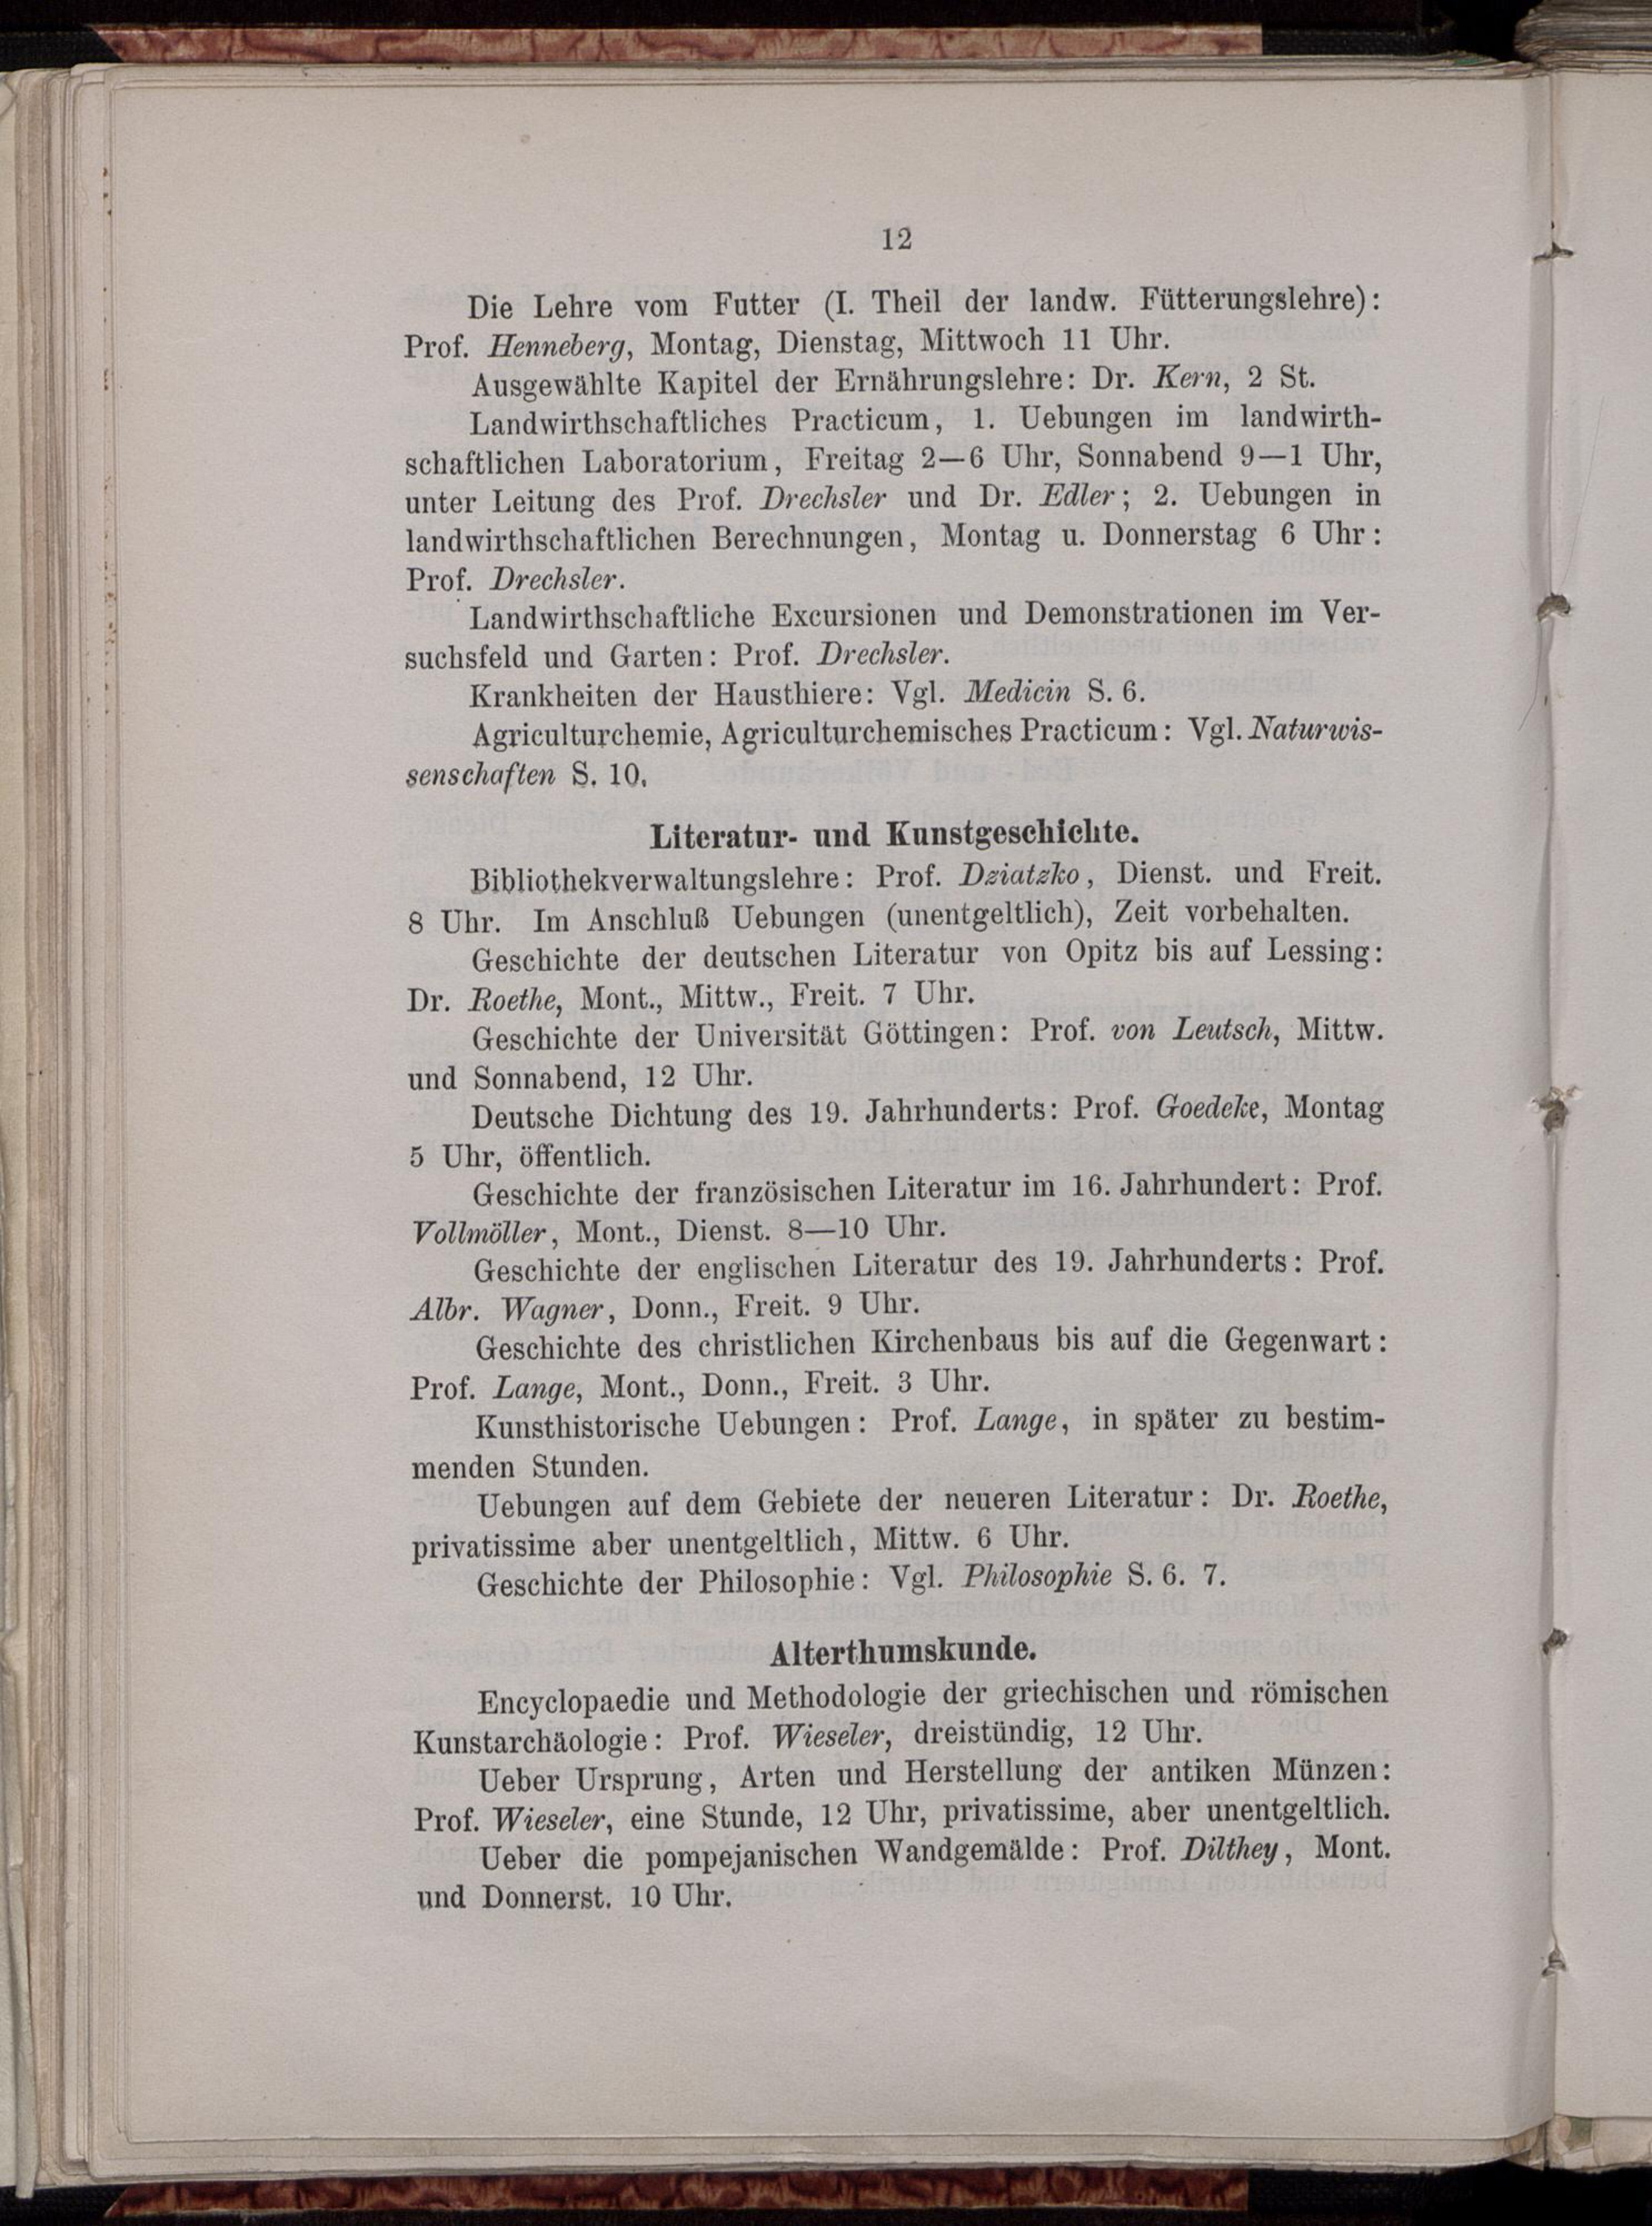
\includegraphics{img/image4.jpg}
\end{center}

Oder ist dies eine offenkundige Zurschaustellung des mitunter als
trocken empfundenen Bibliotheksrufs, die eigentlich eine versteckte
Kritik am Bibliothekswesen ist, die auch im Jahr 2018 noch gelten
sollte? Denn so ganz sicher und geheuer war die Causa Dziatzko der
Bibliothekswelt im Jahr zuvor offenbar nicht, wie man dem Zentralplatt
für das Bibliothekswesen vom November 1886 (Heft 11) in der Rubrik
Personalnachrichten (S. 463) entnehmen kann:

\begin{quote}
\enquote{... Dem Vernehmen nach soll Professor Dr.~Dziatzko
Vorlesungen über bibliothekarische Hilfswissenschaften halten.}
\end{quote}

\begin{center}
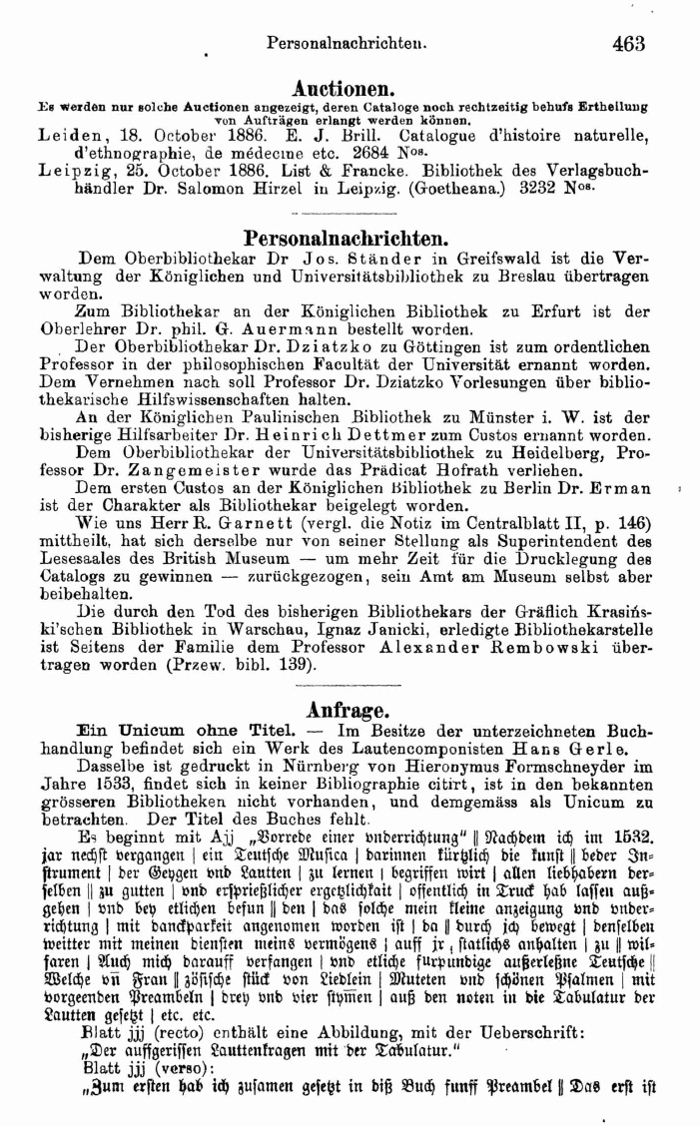
\includegraphics{img/image5.jpg}
\end{center}

Es lässt sich über die zeitbeugenden Eigenschaften der
bibliothekarischen Forschung zum Beispiel in Margrit Bornhöfts Arbeit
von 1999 \enquote{Bibliothekswissenschaft in Deutschland. Eine
Bestandsaufnahme} (Aachen: Verlag Mainz) mehr erfahren. Seien wir
gespannt, ob wir bis zum 100. Jubiläum im Jahr 2028 weitere Erkenntnisse
erfahren können.

%autor
\begin{center}\rule{0.5\linewidth}{\linethickness}\end{center}

\textbf{Prof.~Dr.~Wolfram Horstmann} ist seit 2014 Direktor der SUB
Göttingen und seit 2017 Honorarprofessor am Institut für Bibliotheks-
und Informationswissenschaft der Humboldt-Universität zu Berlin. Nach
seinem Studium der Neurowissenschaften mit informatischer und
wissenschaftstheoretischer Prägung und Promotion zum Thema ``Explaining
Brains by Simulation'' an der Universität Bielefeld war er Leiter der
Publikationsdienste im Hochschulbibliothekszentrum des Landes
Nordrhein-Westfalen (hbz) und Projektmanager des EU-geförderten Projekts
\enquote{Digital Repository
Infrastructure Vision for European Research (DRIVER-II)} an der SUB
Göttingen. Anschließend war er als Chief Information Officer an der
Universität Bielefeld und als Vizedirektor der Bodleian Libraries an der
Universität Oxford tätig.

\end{document}
